\documentclass{article}
\usepackage[utf8]{inputenc}
\usepackage{graphicx}
\usepackage{amsmath}
\usepackage{amsfonts}
\usepackage{hyperref}
\usepackage{color}

\setlength{\parindent}{0em}
\setlength{\parskip}{0.5em}

\title{Bird embedding}
\author{Li-Ping Liu}
\date{}


%%%%%%%%%%%%%%%%%%%%%%%%%%%%%%%%%%%%%%%%%%%%%%%%%%%%%%%%%%%%%%%%%%%%%%%%%%%%%%%%%%%%%%%%%%
% some notations
\newcommand{\wt}{\boldsymbol{\rho}}
\newcommand{\obswt}{\boldsymbol{\beta}}
\newcommand{\emb}{\boldsymbol{\alpha}}

%%%%%%%%%%%%%%%%%%%%%%%%%%%%%%%%%%%%%%%%%%%%%%%%%%%%%%%%%%%%%%%%%%%%%%%%%%%%%%%%%%%%%%%%%%
\begin{document}

\maketitle

\section{Introduction}

The eBird data consists of checklists of bird observations. The figure below shows some sites having checklist submissions on Manhattan island. eBird project even includes a \href{http://ebird.org/ebird/livesubs}{\textcolor{blue}{webpage}} that shows real-time submissions. 


\begin{figure}[h]
    \centering
    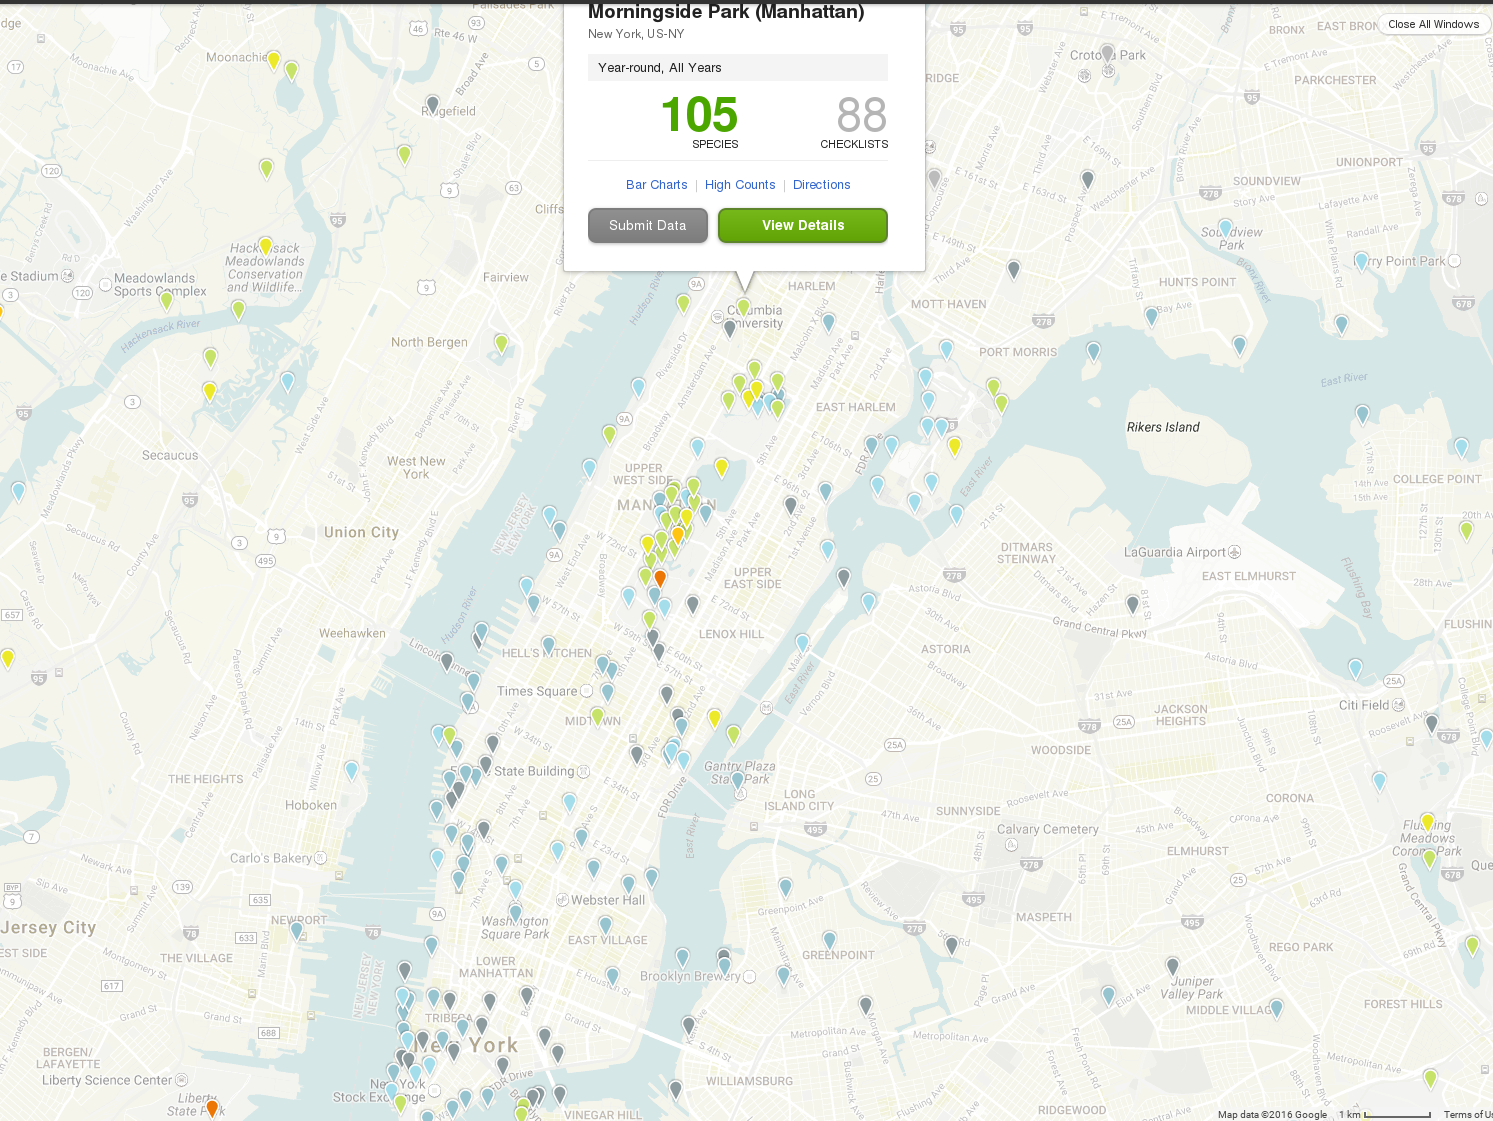
\includegraphics[width=0.8\textwidth]{figures/ebird-checklist-manhattan.png}
    \caption{eBird checklist submissions on Manhattan island. (I believe) Checklists are aggregated by a number of sites for better plot. The location at CU is mistakenly labeled as Morningside Park. Zoom in for better view. }
    \label{fig1}
\end{figure}


Each checklist contains its location (latitude \& longitude), time point, and a list of bird counts for 953 species. Two sets of covariates are associated to each checklist. The first set ($\approx$ 12) of covariates describe the environmental information, such as elevation, temperature, and vegetation coverage, and explain why the bird is there. The second set ($\approx$4) of covariates are about the observation process and states how the observation is made, such as the type of observation (staitionary, traveling, area survey, etc.) and duration of observation. 

There are about 6 million checklists during the last 5 years (from 2010 to 2014). 

In this work, we would like to discover bird relations by bird embedding. The idea of bird embedding originates from word embedding in NLP, where various relations among words are discovered[citation of word embedding]. In this work, we would like to discover relations among birds by applying the embedding technique to the eBird data. 

Dispite its similarity with word embedding, there are new problems to consider for bird embedding. 
\begin{itemize}
\item Large quantity of data, which has 6 millions observations.
\item Rich information about checklists. In another word, checklists are not from the same distribution. We should construct a model in which environmental covariates expain presence/absence of species, and bird embedding captures interactions among species.  
\item Locations near each other should have similar distribution of birds, not only because they share similar covariates, but also because birds fly around. How to smooth the distribution?
\item How can we explain the embedding result? Making recommendation may not be a good idea here. 
\end{itemize}


\section{Bird Embedding}

The first model to consider is the combination of exponential family embedding and the exposure model.

In the embedding model, we essentially need to define the conditional distribution of the bird count of a species in a checklist given its {\it context}. Since we are interested in relationships among bird species, the {\it context} of a bird count is the vector of bird counts of other species in the checklist. Due to the generality of context, we can define the context of a bird count flexibly, for example, as bird counts of other species averaged over checklists within some radius of the current observation. The average may give more stable results, but we will consider this later. 

The exposure model can be used to describe the observation process. Mathematically, it plays the role of down-weighting zero entries in the observation matrix. In another word, a species is not observed either because no such bird lives there or because it is not detected by that observation. If the model choose the second explanation, then model would use little strength to fit the zero value. We will see this after we have defined the model formally.  

Let's define the model. Suppose there are $N$ checklists, and let $i$, $1 \le i \le N$, index checklists. In the data there are $J = 214$ species, each of which is indexed by $j$, $1 \le j \le J$.  
In each checklist $i$, $y_{ij}$ birds are observed for species $j$. 

For each checklist, the feature vector $\mathbf{x}_{i}$ brings some information of the observation process. The probability $u_{ij}$ of observing each species $j$ is calculated as $u_{ij} = \mathrm{logistic}(\obswt_j^\top \mathbf{x}_i + \bar{\beta}_j)$, where $\obswt_j$ is a parameter, and $\bar{\beta}_j$ is the intercept term. The indicator $b_{ij}$ of observing species $j$ at checklist $i$ is sampled from Bernoulli distribution with probability $u_{ij}$. 
\begin{eqnarray}
b_{ij} &\sim& \mathrm{Bernoulli}(u_{ij}).
\end{eqnarray}

The observed count $y_{ij}$ is from Poisson distribution defined as follows. 
\begin{eqnarray}
y_{ij} &\sim& \mathrm{Poisson}(b_{ij} \lambda_{ij}),
\end{eqnarray}
where the rate $\lambda_{ij}$ is the rate calculated from the embedding. 

To define the embedding, we first define the {\it context} of $y_{ij}$, which consists of species with positive observations. 
\begin{eqnarray}
C_{ij} = \{j': y_{ij'} > 0, j' \neq j\}
\end{eqnarray}

The embedding of species $j$ is $\emb_j$. The rate is defined as follows. 
\begin{eqnarray}
\lambda_{ij} &=& f\left(\wt_{j}^\top \sum_{j' \in C_{ij}} r(y_{ij'}) \emb_{j'} + \bar{\lambda}_{j} \right) \label{lambda_exp} 
\end{eqnarray}
The vector $\wt_j$ is the weight vector shared by checklists of species $j$. The function $r(\cdot)$ maps counts to a value in $[0, 1]$ to avoid that a large count dominate the embedding. The function $f(\cdot)$ maps the product from $\mathbb{R}$ to $\mathbb{R}^{+}$. It can be defined as the exponential function or the softplus function ($f(x) = \log(1 + \exp(x))$). Different with traditional embedding, we also include an intercept term $\bar{\lambda}_{j}$ as the base rate.

Gaussian priors are put on the parameters $\alpha_j$, $\rho_j$, and $\beta_j$. 
\begin{eqnarray}
\emb_j &\sim& \mathrm{Normal}(\mathbf{0}, \sigma^2_1 I), \\
\wt_j &\sim& \mathrm{Normal}(\mathbf{0}, \sigma^2_2 I), \\
\obswt_j &\sim& \mathrm{Normal}(\mathbf{0}, \sigma^2_3 I),
\end{eqnarray}
where $\sigma_1^2$, $\sigma_2^2$, and $\sigma_3^2$ are hyper-parameters, $\mathbf{0}$ represents a zero vector with proper length $N$, and $I$ represents the identity matrix of with proper size. 

The parameter $\wt$ and and $\emb$ explains the correlation among bird species. The correlation comes from either shared environmental factors or birds' interactions. If the embedding is to capture more about birds' interactions, the base rate $\bar{\lambda}_{j}$ needs to explain more about environmental factors by including environmental covariates. 


\subsection{Settings}

The model is defined to be flexible. Four different configurations are listed here.  
\begin{itemize}


\item[]{\bf downweighting zeros}: There are three settings for downweighting zeros. The first one is not downweighting zeros, the probability $u_{ij}$ for each $(i, j)$ being set to 1 instead of calculated by the logistic function. The second setting fits the probability $u_{ij}$ by the term $\bar{\beta}$ only, then the distribution of counts is essentially a zero-inflated Poisson distribution. The third setting fits the probability $u_{ij}$ by both observation covariates and $\bar{\beta}$, so zeros a further explained by covariates.    

\item[]{\bf scaling context}: The counts in context exhibit large varince, and counts of some species are much larger than those of others. To prevent the embedding being dominated by species with large counts, counts are normalized by $r(\cdot)$ function. One method is to divide each count by the 95\% quantile of the counts of that species. If the setting is on, the counts are scaled.

\item[]{\bf intercept term:} $\bar{\lambda}_{j} = 0$ gives the basic embedding, or $\bar{\lambda}_{j}$ is fit by the data. 

\item[]{\bf link function:} $f(x) = \exp(x)$, or $f(x) = \log(1 + \exp(x))$.
\end{itemize}

\section{Inference}

In this section, we develop a varitional inference method to infer parameters of the model. The inference method below is general enough to include all settings above.

\subsection{ E-step: calculating posterior distribution of observation variable}

In this subsection, we calculate the posterior distribution of $b_{ij}$.
\begin{eqnarray}
q_{ij}^{0} &=& p(b_{ij} = 0 | y_{ij} > 0, \lambda_{ij}, u_{ij}) =  0 \\
q_{ij}^{1} &=& p(b_{ij} = 1 | y_{ij} > 0, \lambda_{ij}, u_{ij}) =  1 \\[10pt]
q_{ij}^{0} &=& p(b_{ij} = 0 | y_{ij} = 0, \lambda_{ij}, u_{ij}) =  \frac{1 - u_{ij}}{1 - u_{ij} + u_{ij}\exp(-\lambda_{ij})} \\
q_{ij}^{1} &=& p(b_{ij} = 1 | y_{ij} = 0, \lambda_{ij}, u_{ij}) =  \frac{u_{ij}\exp(-\lambda_{ij})}{1 - u_{ij} + u_{ij}\exp(-\lambda_{ij})}
\end{eqnarray}


\subsection{M-step: maximizing the log-likelihood with respect to model parameter}

In the M-step, we want to maximize the following objective.
\begin{eqnarray}
LL(\wt, \emb, \obswt) &=& \sum_{ij} E_{b_{ij}} \Big[\log p\left(y_{ij} | b_{ij} \lambda_{ij} \right) + \log p\left(b_{ij} | \obswt_j^\top \mathbf{x}_{ij}\right)\Big] \nonumber\\
&=& \sum_{ij}  - q_{ij}^0 \log (1 +  \exp(\obswt_j^\top \mathbf{x}_i)) \mathbb{I}[y_{ij}=0] + q_{ij}^1 \Big( y_{ij}\log(\lambda_{ij}) - \lambda_{ij} - \log \big(1 + \exp( - \obswt_j^\top \mathbf{x}_i) \big) \Big) \nonumber
\end{eqnarray}

Take derivatives with respect to the parameters. 
\begin{eqnarray}
\nabla_{\wt_j} LL &=& \sum_{i}  q_{ij}^1 \left( y_{ij}/\lambda_{ij} - 1 \right)
\nabla_{\wt_j} \lambda_{ij} \\
\nabla_{\emb_j} LL &=& \sum_{i}\sum_{j' \in C_{ij}}  q_{ij'}^1 \left( y_{ij'}/\lambda_{ij'} - 1 \right)
\nabla_{\emb_j} \lambda_{ij'} \\
\nabla_{\obswt_j} LL  &=& \sum_{i} - q_{ij}^0 \mathrm{logistic}(\obswt_j^\top \mathbf{x}_{ij}) \mathbf{x}_{ij} + q_{ij}^1 (1 - \mathrm{logistic}(\obswt_j^\top \mathbf{x}_{ij})) \mathbf{x}_{ij}
\end{eqnarray}

With the softplus function, 
\begin{eqnarray}
\nabla_{\wt_j} \lambda_{ij} &=& \frac{\exp(h_{ij})}{1 + \exp(h_{ij} / \delta)} \sum_{j' \in C_{ij}} r(y_{ij'}) \emb_{j'}, \\
\nabla_{\emb_{j}} \lambda_{ij'} &=& \frac{\exp(h_{ij'})}{1 + \exp(h_{ij'} / \delta)}  r(y_{ij}) \wt_{j'},
\end{eqnarray}
where $h_{ij} = f^{-1}(\lambda_{ij})$.



\subsection{Maximization with Stochastic Gradient}

Combining the E-step with the M-step by appying $q$ values to the gradients above gives the gradient of the log-likelihood with respect to model parameters. 
Instead of calculating the exact gradient with all training instances, we only calculate a noisy gradient by using only one instance randomly drawn from the 
training set. Then we use AdaGrad to update model parameters with noisy graidents. Practically, the algorithm converges within 100,000 iterations. 

\section{Experiment}

In the experiment, a subset of checklists are taken from a rectangular area that mostly overlps with Pennsylvania and the period from day 180 to day 210 in 2014. The 
subset has  overall 5488 checklists (trips)
and 214 bird species (items). The dataset is randomly split into two thirds as the training set and one third as the test set. The model is trained on the training set and tested on the test set for ten times on 10 different random splits. In each training run, the model is optimized on nine tenth of the training set and validated on the rest one tenth. For each random split, the negative predictive log-likelihood is recorded. In two randomly splits, there are some outliers that greatly affect the performance of the model, so these two random splits are removed. We report the average negative predictive log-likelihood on 8 random splits.

The basic setting is as follows. $K = 10, \sigma_1 = \sigma_2 = \sigma3 = 100, \bar{\lambda}_j = 0, f(\cdot) = \exp(\cdot)$. Counts in context are scaled by 95\% quantile value of each species. Observation covariates and $\bar{\beta}$ are used to fit $u_{ij}$. In the following result, only the setting to be examined is varied. 

{\bf Downweighting zeros:} See results in Fig.~\ref{fig_dwz}. This result shows that the average performance with different measures of downweighting zeros. When both covariates and $\bar{\beta}$ are used, the mean value of the performance is smallest.   

\begin{figure}[t]
    \centering
    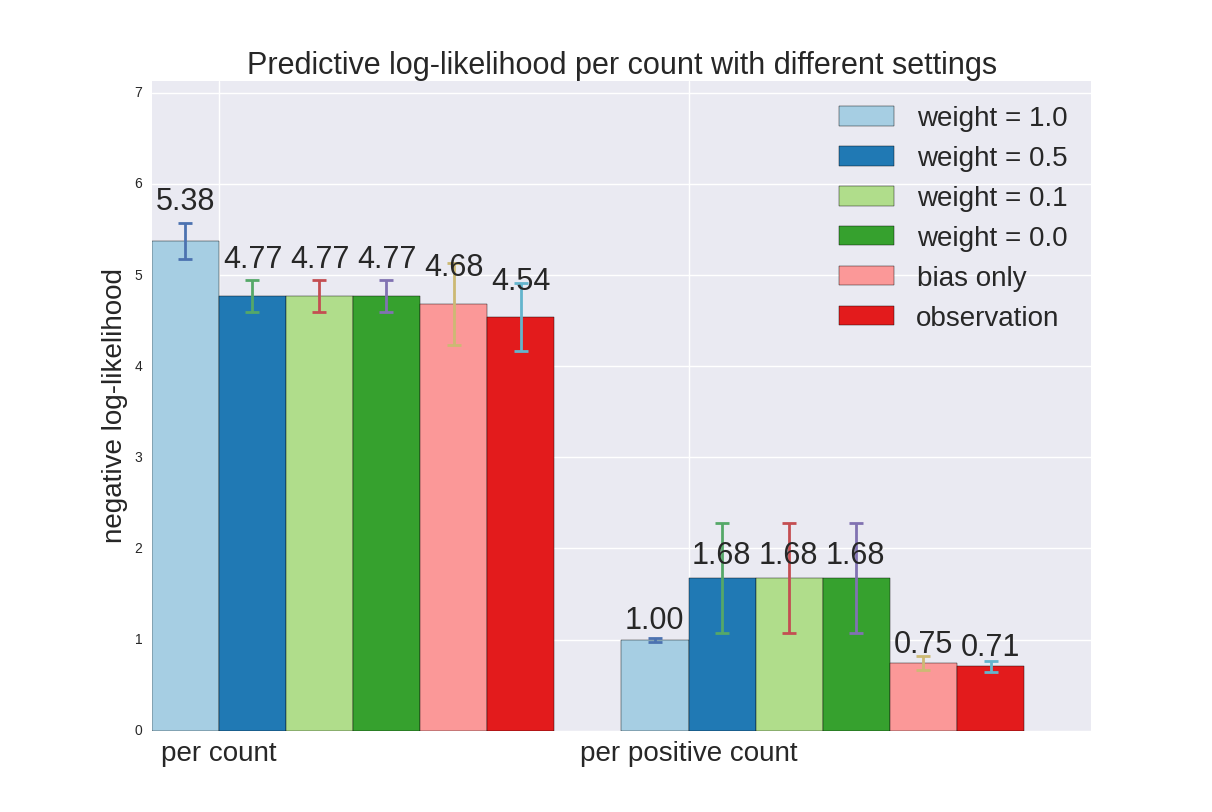
\includegraphics[width=0.6\textwidth]{figures/dwz.png}
    \caption{Negative predicted log-likelihood with different measures of downweighting zeros}
    \label{fig_dwz}
\end{figure}


{\bf Scaling context:} See results in Fig.~\ref{fig_scaling}. Scaling counts in contexts helps to stablize the algorithm. Without scaling the context counts, the log-likelihood of validation set stops increasing before much less iterations than that of the setting with scaling counts. 
\begin{figure}[t]
    \centering
    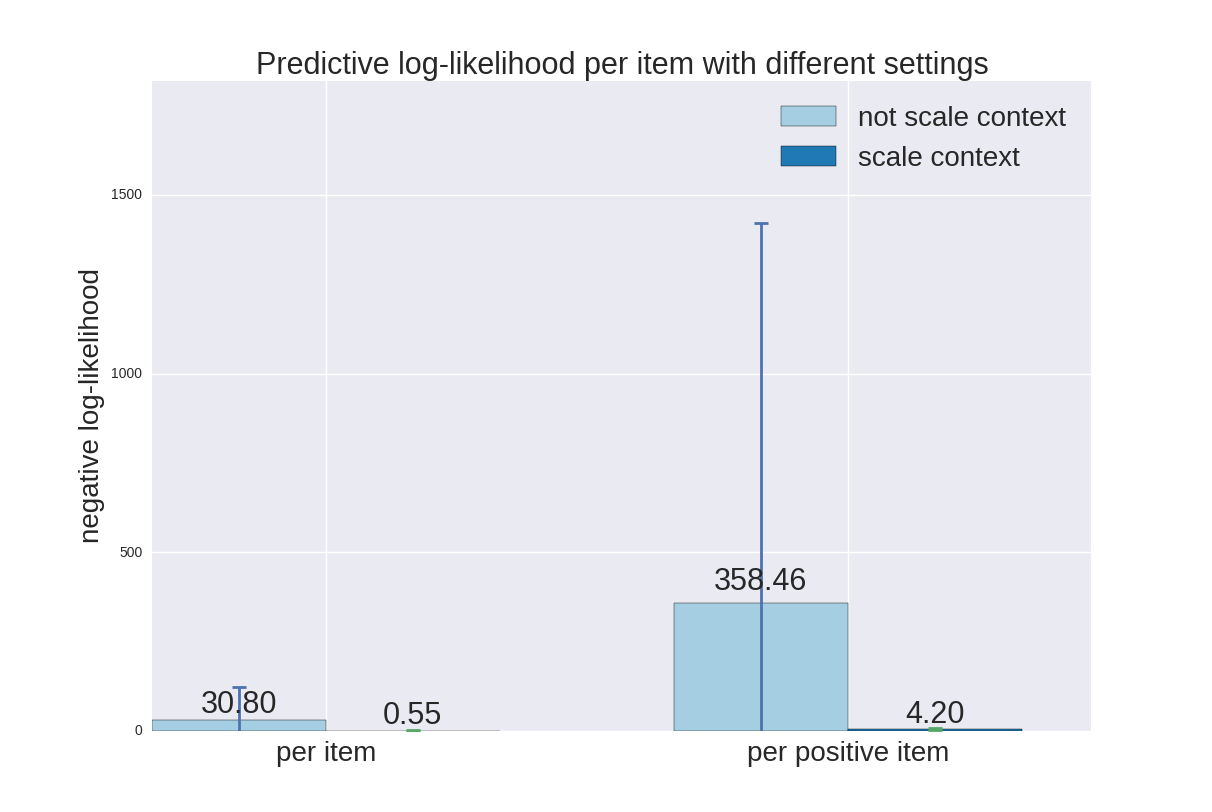
\includegraphics[width=0.6\textwidth]{figures/scale_context.png}
    \caption{Negative predicted log-likelihood with and without scaling the context}
    \label{fig_scaling}
\end{figure}


{\bf Intercept term: } See results in Fig.~\ref{fig_intercept_term}. Intercept terms $(\bar{\lambda}_j)_j$ helps to explain the data. 
\begin{figure}[t]
    \centering
    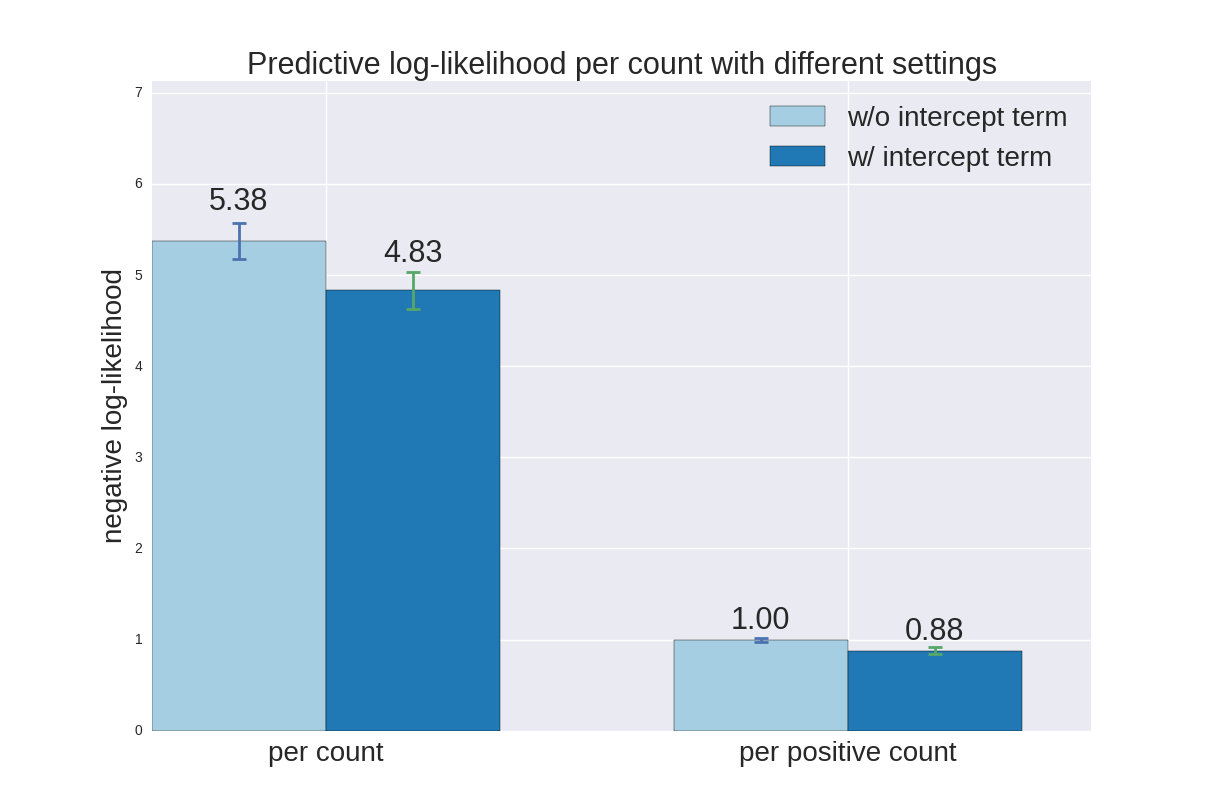
\includegraphics[width=0.6\textwidth]{figures/intercept_term.png}
    \caption{Negative predicted log-likelihood with and without the intercept term}
    \label{fig_intercept_term}
\end{figure}



{\bf : } See results in Fig.~\ref{fig_link_func}. Two link functions give very similar results. 
\begin{figure}[t]
    \centering
    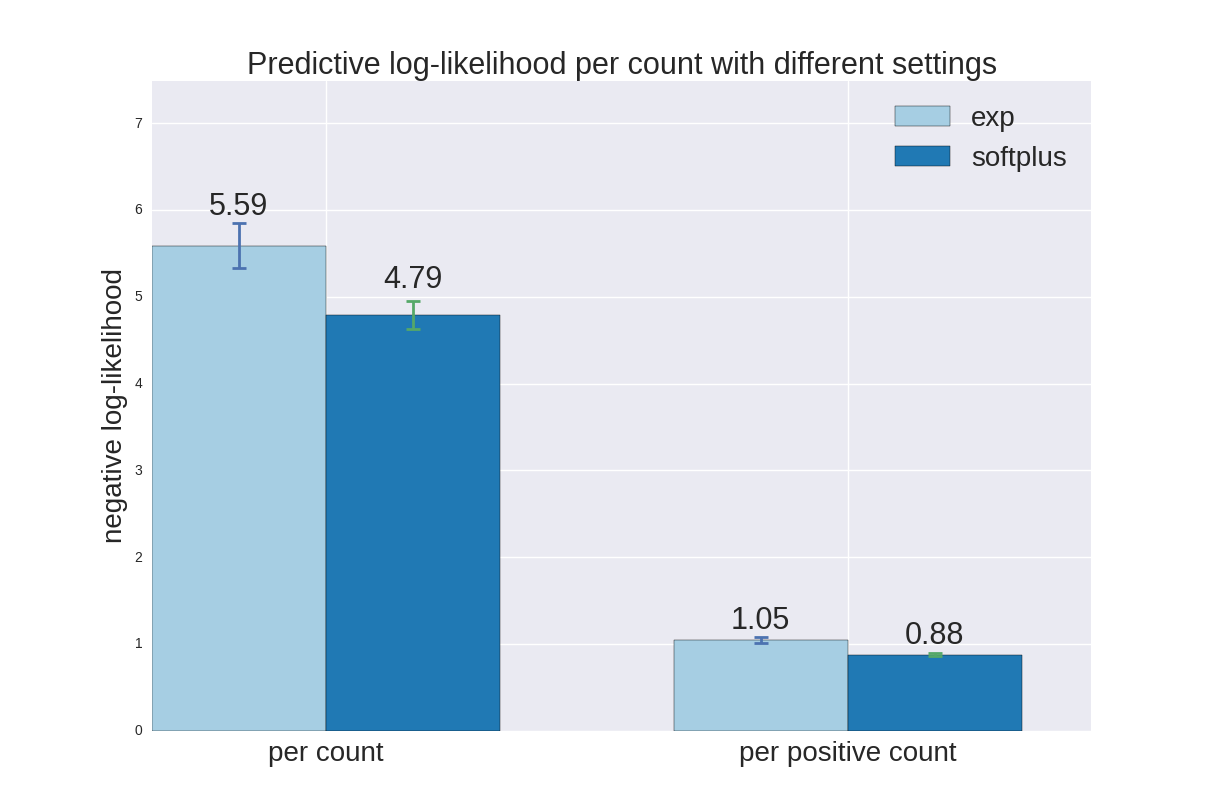
\includegraphics[width=0.6\textwidth]{figures/link_func.png}
    \caption{Negative predicted log-likelihood with $\exp$ and $\mathrm{softmax}$ as the link function}
    \label{fig_link_func}
\end{figure}

\begin{figure}[t]
    \centering
    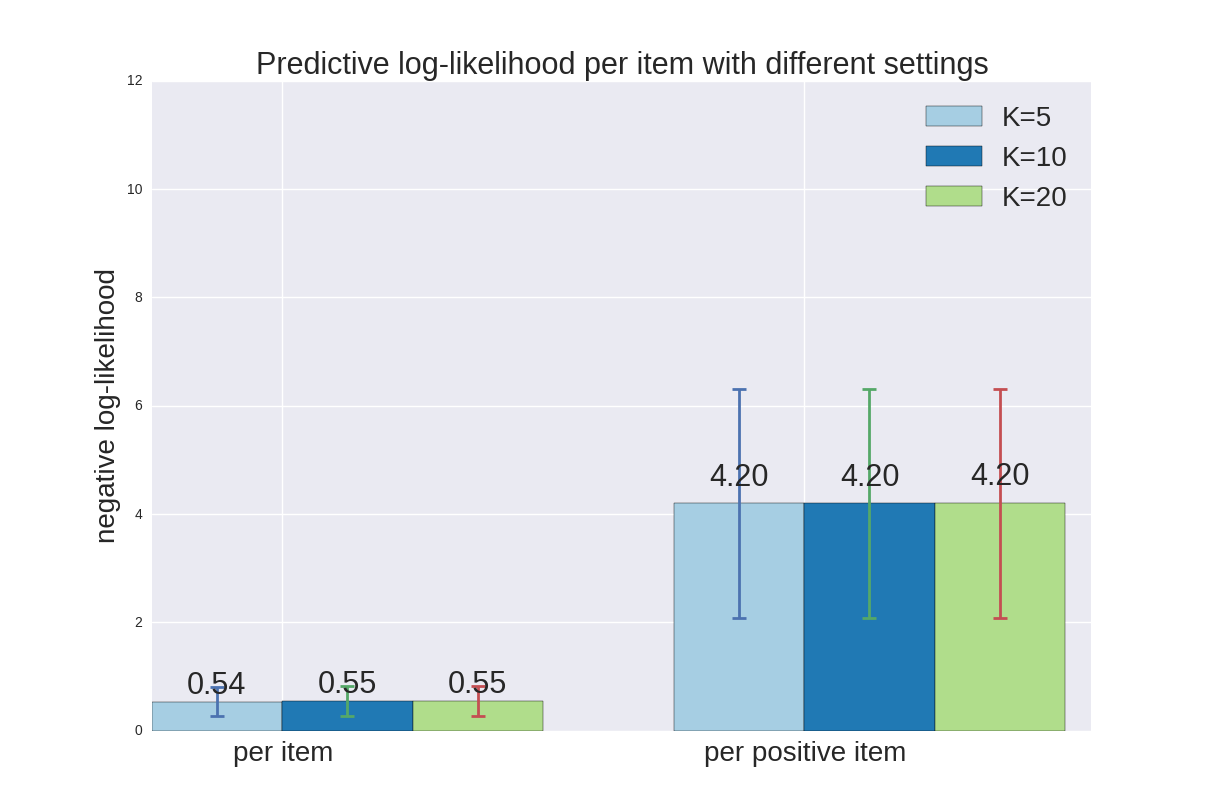
\includegraphics[width=0.6\textwidth]{figures/variate_K.png}
    \caption{Negative predicted log-likelihood with different dimensionalities}
    \label{fig_dimensionality}
\end{figure}



\section{Research Directions}

Assumption: embeddings at similar time-locations are similar but different. Can we use a $\wt_{ij}$ for each checklist $i$ and species $j$ and put a GP prior over $\wt_{ij}$-s to encourage strong correlation among $\wt_{ij}$-s at neighboring locations?  

Can we predict the presence/absence of species?


\end{document}

